\documentclass[conference]{IEEEtran}
\usepackage{cite}
\usepackage{amsmath,amssymb,amsfonts}
\usepackage{algorithmic}
\usepackage{graphicx}
\usepackage{textcomp}
\usepackage{url}

\def\BibTeX{{\rm B\kern-.05em{\sc i\kern-.025em b}\kern-.08em
    T\kern-.1667em\lower.7ex\hbox{E}\kern-.125emX}}
\begin{document}

\title{Parallel Compilation in the Cloud}

\author{\IEEEauthorblockN{Jamie Willis (13353)}
\IEEEauthorblockA{\textit{School of Computer Science} \\
\textit{University of Bristol}\\
jw14896@bristol.ac.uk}
\and
\IEEEauthorblockN{Samuel Russell (14591)}
\IEEEauthorblockA{\textit{School of Computer Science} \\
\textit{University of Bristol}\\
sr14978@bristol.ac.uk}
}

\maketitle

\begin{abstract}
We present an application based in the cloud allowing users to compile large C
or C++ projects in parallel, utilising Google App Engine (GAE). The application
can compile projects by allowing a user to upload a flattened zip with the
source code and headers. It is available online at

\noindent\url{https://cloudcomputingcompiler.appspot.com}.

\end{abstract}
\section{Introduction}
In industry, very large C or C++ projects are common. These can take a very
long time to compile using GCC, and this is a
large waste of time for developers. Many compilers are not multi-threaded - the
process of compilation and optimisation must be done in an ordering
with many dependencies. Despite this, however, each file in itself is completely
orthogonal to every other file (until link-time). This results in an ability to
compile multiple files at once by using scripts that launch many compiler
instances in separate threads. This is a good improvement on the compilation
process, but it is limited by the number of processor cores you have.
Additionally, if your compiler \emph{is} multi-threaded \cite{rust}, this will
place a large amount of strain on the system or prove ineffective, depending on
the type of parallelism it employs.

Our solution is to leverage multiple processors, distributed across the cloud,
each of which can handle the compilation of one or many files depending on how
big the files are. This can prove to be a large advantage for much larger
projects, that might otherwise take over half an hour to compile. This technique
also allows us to leverage multi-threaded compilers whilst also compiling files
in parallel if the hardware allows it.

% potentially add in more information?

\section{Implementation}
\subsection{Overall Procedure}
\begin{figure}[ht] % ht
    \centering
    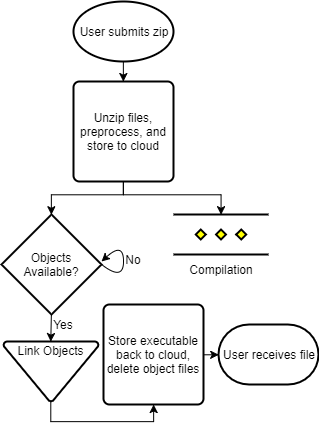
\includegraphics[width=2.4in]{WorkArchitecture.png}
    \caption{Workflow chart}
    \label{fig:overview}
\end{figure}

Figure \ref{fig:overview} illustrates the general workflow, which is now
discussed in more detail. A user visits the website provided by the front end
service. They send a zip file along with the corresponding compiler and linker
flags to the API using the webapp.

Then, in the cloud, the zip file is tagged and uploaded to object storage, a
task is submitted to the queue to initiate the compilation and the tag is
returned to the user app for retrieval of the results.

Upon completion of the compilation, both the results file and executable are
uploaded to object storage and they become available for the app to
download with the warnings presented in browser. If compilation failed, errors
are presented to the user instead.

The compilation process consists of three steps:
Firstly, the zip file is unpacked and the GCC macro pre-processor is ran over
each of the source files to include all necessary headers. This allows us to
discard the header files, removing the need to transfer them \emph{all} to
workers for \emph{every} source file, at the cost of source file size. These
source files are then uploaded to object storage individually and the zip file
is deleted as it is no longer needed. A task for compilation of each file is
then submitted to the queue along with a task to link the resulting object
files together.

Secondly, for each compilation task of a source file, the file is downloaded
from object storage and compiled locally. The object file, along with any
warnings and errors is then collected and stored back to object storage.

Thirdly, the linker checks that all files have been compiled then, if they were
all successful, downloads them in to a local folder before linking them together
in to an executable. If the objects file are not all ready it reschedules
itself and returns. Finally, it uploads the executable or coagulated error
messages so they are available for the user.

\subsection{Underlying Architecture}
\begin{figure}[ht] % ht
    \centering
    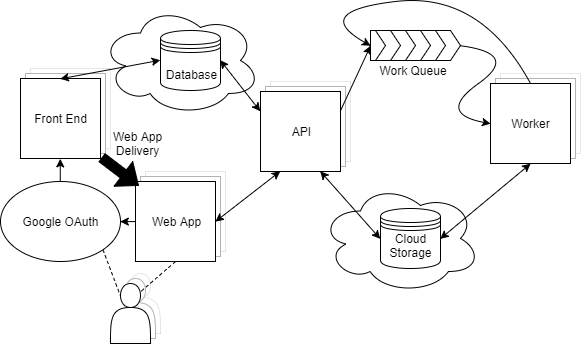
\includegraphics[width=3.2in]{OverallArchitecture.png}
    \caption{Overall architecture}
    \label{fig:underlying}
\end{figure}

Our solution consists of a collection of independent micro services, each
managed separately by Google App Engine. We used this platform-as-a-service
(PaaS) offering to take advantage of Google Flex\cite{GAE} environment which
automatically scales instances and load balances requests. In the flex mode of GAE,
server instances run inside containers which are created from the uploaded
source code. This use of containers requires that a docker image is constructed,
which can take much longer than executing the server code on its own, but provides a clean
way of managing the running instances and, later, creation of cloned instances
is much faster.

There are three micro-services, each of which is written in Python using the
Flask web framework \cite{Flask}:
\begin{itemize}
\item A Front-end service which provides users access to web
pages including static and dynamic content.

\item An API service, which provides
access to all the functionality through a RESTful interface.

\item The third micro-service conducts a \emph{map-then-reduce} process to
compile the given source code and store it to object storage.
\end{itemize}

We could have created three micro-services to perform the third operation - an
individual unzip, compile and link process - however, we opted to use one
micro-service for all three since this means the workers are more flexible; they can complete any
of the actions so fewer instances will be needed for light loads.

To create a micro-service, a \texttt{yaml} file must be submitted defining
how GAE should respond to requests, giving details of the runtime of the
app instance and defining the start up command. We utilised
Gunicorn\cite{gunicorn} as the Web Server Gateway Interface to serve up
the web interface. Our folder structure also included a template directory for
serving up dynamic pages and a static directory for the static content like
style sheets. We also uploaded a \texttt{requirements.txt} file to tell the
container build script to pull in the appropriate libraries.

The static content to be served to the user is cached in a geographically
distributed fashion on Google's Content Management System. This did cause some
issues in testing since when uploading a new version, the old code was still
present in the cache so the content did not update. However, in production this
improves the latency of resource retrieval greatly.

To store information about users we have used Google's cloud
Datastore\cite{datastore} offering. All micro-services communicate with the
Datastore through the Google's client API. Datastore is a non-relational
database: structured queries like table joins are not available. However,
it is great for storing simple variable types as it is
massively scalable and delivers high performance due to a distributed
architecture, and scales automatically. However, there are limits to parallel
accesses as many accesses to data on the same data group can lead to contention.
Distributed databases need to consider consistency and Datastore uses
strong consistency when querying keys but eventual consistency for other
content-based queries. This is fine for our application's needs since it is not used for critical data. Like every good database, it guarantees atomic transactions and
encrypts all data written to disk.

All files are stored in Google's Cloud Object storage offering\cite{storage}
which provides a unified place for data across the micro-services. Object
storage differs from other storage architectures like hierarchical file-systems;
it consists of an unstructured collection of variable sized object blobs each
retrievable by a globally unique identifier - in Google Cloud storage you can
create folders, but they are just abstractions over globally unique names.
We created our own object storage bucket to store our zip files, source code, 
object code and compiler messages.

The API service is decoupled from the worker service using a Google's PubSub
queue\cite{pubsub}. We use a push queue that instigates the jobs by submitting
POST requests to the worker service. It can protect the workers from large
surges in demand using flow control dynamic rate limiting. Also, it improves
robustness since it guarantees \emph{at-least-once} messaging by re-scheduling
failed jobs.

We could have also used Google's MemCache\cite{mem} offering which provides a
much faster, local but smaller storage option to the web servers. Inside the
memory cache, data is held in RAM and so, when used to store frequently accessed
data, it can improve performance and therefore cost. However, care must be taken
to decide what to put into the cache and on the free tier there are no
guarantees about the data still being there when you next need it; it may
be cleared at any time to make space for another application. This means
it is only really appropriate for static content.

We included user accounts on the application so users can check up on previous
compilations and download the resulting executables. For this, we integrated
with Google's identity API using \texttt{OAuth2}; we used a flask
plugin called \texttt{UserOAuth2}\cite{oauth} to redirect to Google's
authentication page and handle the response token by looking up the user details 
on Google+, such as name and user id number.

After a user has logged on, we want to store their credentials so that we can
customise their experience. We found the simplest way to achieve this in a
distributed system is to store them in the user's browser; they will get sent
with each request identifying who it has come from. Flask's session plug-in
makes this easy and secure by encrypting the information before it is sent and
decrypting it again on receipt.

\section{Scalability}
Vertical scaling involves increasing the size of your compute devices to get
better performance. This normally means the software architecture does not need to be
changed, however, there are limits to the size of servers and also, using many
smaller commodity servers is cheaper due to efficiencies of scale. Therefore,
the current trend is to use the horizontal scaling of using more machines to
satisfy high demand.

Howver, it is worth discussing how we \emph{could} have implemented vertical
scaling and why it is likely not advantageous with respect to further
enhancements we could make. Vertical scaling can be realised by making use of
more resources on each of our worker threads. This is trivially achievable with
our application by shipping $n$ source files to each worker where $n$ is the
number of cores on the machine. Then we would spawn off $n$ at once instances of
the compiler. This was the approach discussed in the introduction. However, this is
not a suitable idea for two reasons: it falls short with regard to
multi-threaded compilers, which are already utilising any available extra power;
it relies on the servers provided to us being multi-core, which is less likely
to be available to us in the commodity-heavy infrastructure we described.

There are three axis of the horizontal scaling cube, and Google App Engine
implements them all:

\begin{itemize}
\item Scaling out is achievable with functional decomposition, which we have
done by splitting our system into three micro-services. This creates good software
maintainability; each part of the process is decoupled from the next and
so has clear, well-defined interaction points.

\item The second is data-partitioning, which can be geographical or purely over
separate user demographics. Since, within our application, users do not share
data and usually with remain in one location for sustained periods of time,
assigning resources in close proximity to users will increase performance as
instance caches become more efficient. GAE will create multiple server 
instances from our template in different data centres and can route traffic to
the most applicable one.

\item Finally, within a specific feature and geographic server group there can
be instance replication to serve the load. This replicated instance group can also
be scaled up and down to match demand as close as possible. GAE support three
types of scaling: Manual, Basic and Automatic. In manual scaling mode, the
service administrator or management software decides when to increase or
decrease the number of instances. The instances have a persisting state and are
good for long running jobs but are not as reactive to change in load. Basic
scaling only creates a new instance when the application receives a request and
remove again after it has finished. This is targeted towards very intermittent,
small-scale use as it uses minimal resources, but has the overhead of starting
up new instances for new requests. Automatic scaling uses application metrics 
such as request latencies to gauge scaling demands. We use GAE automatic
scaling between one and sixteen instances based on the CPU utilisation to
provide a capable but responsive system.
\end{itemize}

You can also host multiple versions of software and do incremental feature
rollouts by using traffic splitting to gradually upgrade the service with
minimal disruption.

\section{Future Work and Limitations}
\subsection{Linux Only Compilation}
A severe current limitation of our system is that it only supported Linux
compilation, since the server we are provided with is a Linux server. In order
to compile for Windows and other platforms, we would need to compile our own
cross-compilers for GCC that run on Linux but target other platforms, which is
quite involved. For this proof of concept, however, this is not deemed to be a
requirement.
\subsection{More Languages}
Currently, only C and C++ are supported languages. However, it would be possible
in future work to include more languages that suffer from the same long
compilation times. The limitation would be on what compilers are installed on
the server, and whether or not we could install new ones.
\subsection{Non-nested Zip Structure}
A current limitation with the design is the requirement of a flattened zip
structure for the uploaded source code. Ideally in future the app would be able
to support any folder structure inside the zip and create the appropriate
structure in the blob storage. This should not be too difficult to achieve, but
we decided it does not add much to the application given that the main focus is
on the parallel aspect.
\subsection{New Compilers}
The current implementation of this application only allows us to make use of GCC
and G++ compilers. Ideally, we would also like to support the MSVC compiler and
Clang. The former is an example of a compiler that already performs
multi-threaded compilation by instantiating itself multiple times \cite{MSVC},
so wouldn't benefit from running it multiple times in parallel as suggested in
the introduction.
\section{Conclusion}
In this paper we have presented a means to compile large projects whilst
leveraging the scalable power of a cloud platform using micro-services. We have
made a working prototype that horizontally scales to
meet both user demand and reach performance goals for per user job submitions.
The level of parallelism that this application can achieve is likely to outweigh
the performance observed with the naive multi-threaded approach for large
projects - the performance will obviously not outperform a serial approach for
small projects, with overhead for communication.
The application is available online at
\textbf{\url{https://cloudcomputingcompiler.appspot.com}}.
The application is bundled with an example zip file you can submit to the app.
You should use G++ with the C++ 11 standard. In addition you are required to provide
the following linker flag: \texttt{-pthread}. It is recommended to also use
\texttt{-O3 -pedantic -Wall} as the compiler flags. The executable returned can
be ran, if desired, on a Linux terminal with \texttt{./a.out
hello\_world.stdc}, a sample program included with the source code.

\begin{thebibliography}{00}

\bibitem{rust}
    Rust Compiler - Parallel Code Generation
    \url{https://internals.rust-lang.org/t/default-settings-for-parallel-codegen/519}


\bibitem{GAE}
    Google App Engine: A PaaS offering auto scaling instances
    \url{https://cloud.google.com/appengine/docs/flexible/}

\bibitem{Flask}
    Flask: a web microframework for Python
    \url{http://flask.pocoo.org/}

\bibitem{gunicorn}
    Gunicorn: a Python WSGI HTTP Server for UNIX
    \url{http://gunicorn.org/}

\bibitem{datastore}
    Google Cloud Datastore: a Highly Scalable NoSQL Database
    \url{https://cloud.google.com/datastore/}

\bibitem{storage}
    Google Cloud Storage: a Unified Object Storage
    \url{https://cloud.google.com/storage/}

\bibitem{pubsub}
   PubSub: Google Task Queue
    \url{https://cloud.google.com/pubsub/}

\bibitem{mem}
   Effective MemCache
    \url{https://cloud.google.com/appengine/articles/scaling/memcache/} 

\bibitem{oauth}
   OAth2 Flask extension
    \url{http://oauth2client.readthedocs.io/en/latest/source/oauth2client.contrib.flask_util.html}

\bibitem{MSVC}
 	Multi-process compilation using \texttt{-MP} MSVC
 	\url{https://msdn.microsoft.com/en-us/library/bb385193.aspx}

\end{thebibliography}
\end{document}
